\documentclass[10.5pt,a4paper]{article}
\usepackage[a4paper,left=2.6cm,right=2.6cm,top=2.6cm,bottom=2.5cm]{geometry}
\usepackage{fontspec}
\usepackage{xeCJK}
\setCJKmainfont{AR PL SungtiL GB}[AutoFakeBold=2.5]
\setCJKsansfont{AR PL SungtiL GB}[AutoFakeBold=2.5]
\usepackage{xcolor,graphicx,booktabs,array,amsmath,titlesec,enumitem,caption,float,indentfirst}
\titleformat{\section}{\bfseries\large}{\thesection}{.7em}{}
\titleformat{\subsection}{\bfseries\normalsize}{\thesubsection}{.6em}{}
\titlespacing*{\section}{0pt}{1.4em}{.6em}\titlespacing*{\subsection}{0pt}{1em}{.4em}
\pagestyle{plain}
\renewcommand{\figurename}{图}\renewcommand{\tablename}{表}
\captionsetup{font=small,labelfont=bf,labelsep=quad,skip=4pt}
\setlist[itemize]{leftmargin=1.6em,itemsep=1pt,topsep=2pt,parsep=0pt}
\setlist[enumerate]{leftmargin=1.8em,itemsep=1pt,topsep=2pt,parsep=0pt}
\setlength{\parindent}{2em}\setlength{\parskip}{0pt}\linespread{1.25}
\renewcommand{\arraystretch}{1.15}
\newcommand{\bv}[1]{\textbf{#1}}
\begin{document}

\begin{center}{\LARGE\bfseries 稀疏观测下基于无条件扩散先验的循环数据同化\par}\vspace{.4em}{\large Rayleigh--B\'enard 对流实验汇报\par}\end{center}

\begin{center}\textbf{摘\quad 要}\end{center}
\begingroup\small\leftskip=2em\rightskip=2em
数值求解器的预报含有模型误差，观测稀疏且带噪声。在二维 Rayleigh--B\'enard 对流上，以求解器生成的数据作为真值，从中抽取带噪声的稀疏观测。无条件训练的扩散模型作先验，求解器预报（背景场）与稀疏观测都作为引导项，经扩散后验采样（DPS）逐帧循环同化，并与 20 成员 EnKF 和纯预报比较。预报求解器的 Rayleigh 数取 $5\times10^4$（真值 $10^5$），观测为 1\% 格点、标准差 0.1 的高斯噪声。EnKF 的初始集合取同一轨迹真值前 20 帧各自积分到第 40 帧，从第 40 帧起评价第 40--99 帧，测试 20 个轨迹、3 个随机种子。结果：观测间隔 $K=1$ 与 $K=5$ 时扩散同化的未观测点 RMSE 比 EnKF 低 32\% 与 12\%；$K=10$ 与 $K=20$ 时反而高 13\% 与 22\%。EnKF 的初始集合由测试轨迹真值的前 20 帧积分得到，扩散同化不使用这部分信息。
\endgroup

\section{研究目的}
同化把含误差的预报与稀疏、带噪声的观测结合起来。实验采用的同化方法是：先验只在状态上无条件训练，不接触观测与背景；同化时，求解器的预报作为背景场、观测作为另一项似然，二者都以引导项的形式进入扩散后验采样（Diffusion Posterior Sampling，DPS），逐帧循环，记为\textbf{扩散同化 (DPS)}。对照基线为 EnKF，参照为纯预报（不再同化）。

实验考察：观测间隔 $K$（每 $K$ 帧提供一次观测）增大、观测更稀疏时，扩散同化相对 EnKF 的精度如何变化。

\section{数据设置和处理}
\subsection{控制方程与数值求解}
研究对象为二维 Boussinesq Rayleigh--B\'enard 对流，状态为浮力 $b$ 与速度 $\mathbf u=(u_x,u_z)$：
\begin{equation}
\nabla\!\cdot\!\mathbf u=0,\quad \partial_t b-\kappa\nabla^2 b=-\mathbf u\!\cdot\!\nabla b,\quad \partial_t\mathbf u-\nu\nabla^2\mathbf u+\nabla p-b\,\mathbf e_z=-\mathbf u\!\cdot\!\nabla\mathbf u,
\end{equation}
其中 $\kappa=(\mathrm{Ra}\,\mathrm{Pr})^{-1/2}$，$\nu=(\mathrm{Ra}/\mathrm{Pr})^{-1/2}$。Rayleigh 数 Ra 是方程中的一个无量纲系数，表示浮力驱动与黏性、热扩散耗散之比，数值越大对流越剧烈；Prandtl 数 Pr 取 1。$x$ 方向周期（$L_x=3$），$z$ 方向为上下壁面（$L_z=1$），$b(0)=1$、$b(L_z)=0$，壁面无滑移。用 Dedalus v3 求解（$x$ 方向 Fourier、$z$ 方向 Chebyshev，网格 $72\times24$，时间步长 $\mathrm{d}t=0.01$）。保存的相邻两帧相隔 35 个求解器步（0.35 个时间单位）。

\subsection{数据集}
真值数据的 Ra$=10^5$。数据按轨迹划分，每个轨迹 100 帧，状态形状 $72\times24\times3$（$b$、$u_x$、$u_z$），三个通道的标准差分别为 0.256、0.164、0.158。
\begin{table}[H]\centering\small\caption{数据集划分与用途。}
\begin{tabular}{lccp{7.6cm}}\toprule
子集 & 轨迹数 & 帧数/轨迹 & 用途\\\midrule
训练集 & 160 & 100 & 训练扩散先验\\
验证集 & 20 & 100 & 选取扩散同化的引导参数与 EnKF 的膨胀系数\\
测试集 & 20 & 100 & 仅用于最终评价\\\bottomrule
\end{tabular}\end{table}
数据按通道标准化后用于训练扩散先验，评价在物理量纲下进行。

\section{实验方法}
\subsection{扩散同化 (DPS)}
\textbf{先验。}U-Net（基础通道数 16），在训练集的帧上按标准扩散目标无条件训练 200 个 epoch。训练中不使用观测、背景场和时间信息，同化时不再训练。

\textbf{后验采样与引导。}采样自纯噪声开始（100 步，起始时刻 $t=0.4$），每步在先验得分上叠加三类引导：(1) 观测项，只在观测点上计算，权重由 $\sigma_{\rm obs}=0.05$ 决定；(2) 背景项，在全场计算，约束分析场接近求解器预报，权重由 $\sigma_{\rm bg}=0.3$ 决定；(3) 散度惩罚，系数 0.3。引导总强度系数为 2，不强制观测点取观测值。$\sigma_{\rm obs}$ 是引导强度，不等同于观测噪声标准差。每个窗口取 32 个样本，对每个样本做投影（把速度改写成由流函数导出、壁面处为零的形式，使其严格无散度、壁面无滑移），取样本均值作为分析场，即该帧的同化结果。

\textbf{循环。}同化时刻：用求解器把上一次分析场预报到当前帧作为背景，再采样得到分析场；非同化时刻：直接取求解器预报。起始时刻没有背景，只用该帧观测采样。
\begin{figure}[H]\centering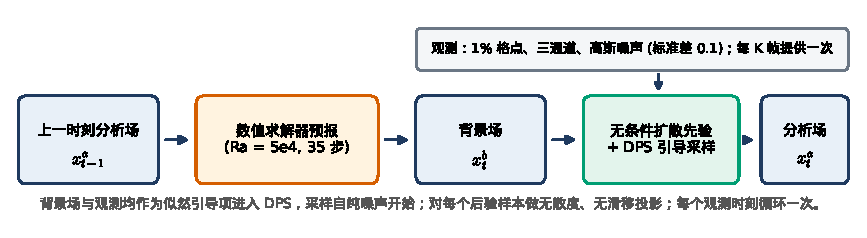
\includegraphics[width=\linewidth]{report_fig_main/workflow.pdf}\caption{扩散同化的循环流程。}\end{figure}

\subsection{对照方法}
\textbf{EnKF。}20 个成员的随机 EnKF，状态为 $(b,u_x,u_z)$ 堆叠的整场向量。分析式为
\begin{equation}
\mathbf x^a-\mathbf x^f=\mathbf P^f\mathbf H^{\!\top}(\mathbf H\mathbf P^f\mathbf H^{\!\top}+\mathbf R)^{-1}[\mathbf y-H(\mathbf x^f)],
\end{equation}
$\mathbf P^f$ 为预报集合的样本协方差，$\mathbf H$ 取观测点，$\mathbf R=0.01\,\mathbf I$（观测误差标准差 0.1）。每个成员使用各自叠加 $\mathcal N(0,\mathbf R)$ 噪声的观测，分析场取集合均值。预报协方差做乘性膨胀，不使用局地化。各成员由求解器（与扩散同化相同，Ra$=5\times10^4$）独立预报。

\textbf{EnKF 的初始集合。}集合成员全部相同时协方差为零，观测不起作用，因此成员之间需要有差异。采用滞后积分 (lag)：取同一测试轨迹真值的第 0--19 帧，各自用求解器积分到第 40 帧，得到 20 个成员，各成员的预报时长为 21--40 帧。该集合使用了测试轨迹真值的前 20 帧。

\textbf{纯预报。}只在起始时刻用观测得到分析场，此后只由求解器预报，不再同化。

\section{实验设置}
\subsection{误差来源}
真值由求解器生成的数据给出，观测从真值抽取并加噪声，所有误差指标都相对真值计算。各类误差的设置如下。
\begin{table}[H]\centering\small\caption{误差设置。}
\begin{tabular}{>{\raggedright\arraybackslash}p{3cm}>{\raggedright\arraybackslash}p{9cm}}\toprule
设置对象 & 取值\\\midrule
真值 & Ra$=10^5$ 的求解器数据\\
预报求解器（背景场） & Ra$=5\times10^4$，与真值的差别即模型误差\\
观测点 & 1728 个格点中随机取 17 个（1\%），三个通道都观测\\
观测噪声 & 在观测值上加标准差 0.1 的高斯噪声\\
观测间隔 & 每 $K$ 帧一次，$K=1,5,10,20$\\
起始 & 第 40 帧，只用该帧观测，不用真值\\\bottomrule
\end{tabular}\end{table}
观测噪声约为通道标准差（合并值 0.198）的 51\%；不做同化时预报的 RMSE 约 0.041，约为通道标准差的 21\%。观测噪声每个同化帧重新抽取，观测点位置由随机种子决定、同一轨迹内不变，同一轨迹、同一种子下三种方法使用相同的观测与噪声。

\subsection{起止时刻}
三种方法在同一轨迹、同一种子下使用相同的观测与噪声，从第 40 帧开始，评价第 40--99 帧（共 60 帧）。EnKF 带着 lag 集合从第 40 帧开始同化；扩散同化与纯预报在第 40 帧起始时只用该帧观测，没有历史信息。

\subsection{评价与调参}
指标为\textbf{未观测点 RMSE}：在没有观测的格点上，三个通道合并，计算分析场（非同化帧为预报场）与真值的均方根误差，物理量纲。评价窗口为第 40--99 帧，观测间隔 $K=1,5,10,20$。随机种子 42、43、44，每个种子 20 个测试轨迹，表中为三个种子的均值，误差线为三个种子的最小至最大。EnKF 的膨胀系数在验证集 5 个轨迹上从 1.0--2.0 中选取，$K=1,5,10,20$ 依次为 1.1、1.4、2.0、2.0；扩散同化的引导参数在验证集 $K=1$ 下选定，各 $K$ 共用。

\section{实验结果和分析}
\subsection{观测间隔的影响}
\begin{table}[H]\centering\small\caption{第 40--99 帧未观测点 RMSE（三个种子均值）。``相对 EnKF''为扩散同化的 RMSE 相对 EnKF 的变化，负值表示更低；``更优轨迹数''为 20 个测试轨迹中扩散同化的 RMSE 低于 EnKF 的个数。}
\begin{tabular}{ccccccc}\toprule
$K$ & EnKF 膨胀 & 扩散同化 (DPS) & EnKF & 纯预报 & 相对 EnKF & 更优轨迹数\\\midrule
1 & 1.1 & 0.0158 & 0.0232 & 0.0412 & -32\% & 20/20 \\
5 & 1.4 & 0.0223 & 0.0253 & 0.0412 & -12\% & 19/20 \\
10 & 2.0 & 0.0296 & 0.0262 & 0.0412 & +13\% & 1/20 \\
20 & 2.0 & 0.0356 & 0.0292 & 0.0412 & +22\% & 0/20 \\
\bottomrule\end{tabular}\end{table}
\begin{figure}[H]\centering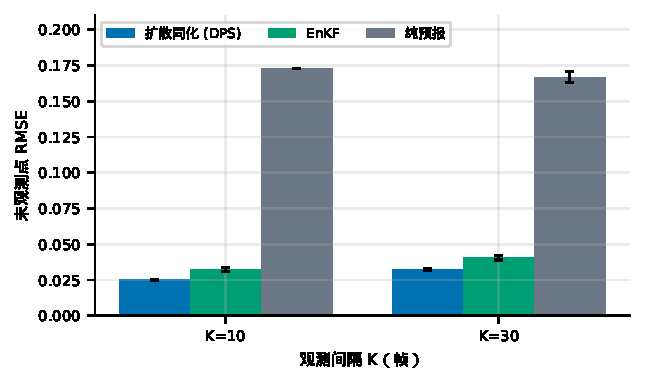
\includegraphics[width=.62\linewidth]{report_fig_main/bar_k.pdf}\caption{不同观测间隔下的未观测点 RMSE（误差线为三个种子的最小至最大）。}\end{figure}
\begin{figure}[H]\centering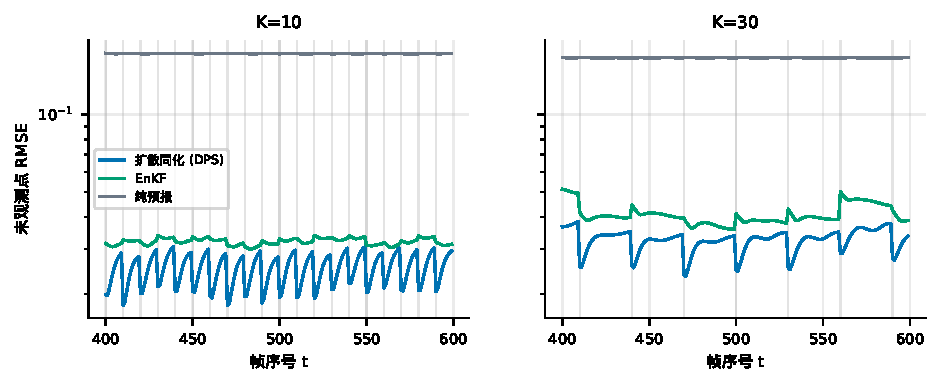
\includegraphics[width=\linewidth]{report_fig_main/curves.pdf}\caption{各观测间隔下的逐帧误差（三个种子、20 个轨迹平均）。}\end{figure}
$K=1$ 和 $5$ 时扩散同化的 RMSE 低于 EnKF，分别低 32\% 与 12\%，20 个轨迹中分别有 20 个与 19 个更优；$K=10$ 和 $20$ 时 EnKF 更低，扩散同化的 RMSE 分别高 13\% 与 22\%，只有 1 个与 0 个轨迹更优。各 $K$ 下两种同化方法都低于纯预报（0.0412）；$K$ 增大时两者都向纯预报靠近。EnKF 的初始集合在第 40 帧的离散度约 0.004，集合均值误差约 0.030。

\subsection{不可压缩约束（散度）}
速度场应满足 $\nabla\!\cdot\mathbf u=0$。用相对散度 $\|\nabla\!\cdot\mathbf u\|/\|\nabla\mathbf u\|$ 衡量（导数用 Fourier--Chebyshev 谱方法计算；真值约 $3.5\times10^{-5}$）。扩散模型的采样输出不满足这一条，扩散同化因此在输出前对速度场做投影（把速度改写成由流函数导出、壁面处为零的形式，使其严格无散度）；EnKF 和纯预报的成员由求解器预报，近似无散度。表~\ref{tab:div} 中``原始输出''是各方法实际给出的结果（扩散同化的结果已经过投影，EnKF 与纯预报没有），``统一投影后''是对三种方法的结果都施加同一个投影之后的值。
\begin{table}[H]\centering\small\caption{同化结果的相对散度（第 40--99 帧，20 个轨迹、3 个种子的均值）。数据取自从第 0 帧起连续同化的运行，其中 EnKF 以扩散同化第 0 帧的结果为中心加扰动初始化，与 5.1 节的运行不同；$K=20$ 的 EnKF 膨胀系数为 1.4。}\label{tab:div}
\begin{tabular}{lcccc}\toprule
 & \multicolumn{2}{c}{$K=1$} & \multicolumn{2}{c}{$K=20$}\\\cmidrule(lr){2-3}\cmidrule(lr){4-5}
方法 & 原始输出 & 统一投影后 & 原始输出 & 统一投影后\\\midrule
扩散同化 (DPS) & $4.2\times10^{-7}$ & $1.2\times10^{-7}$ & $9.9\times10^{-6}$ & $1.3\times10^{-7}$ \\
EnKF & $9.4\times10^{-6}$ & $1.3\times10^{-7}$ & $9.1\times10^{-6}$ & $1.3\times10^{-7}$ \\
纯预报 & $9.2\times10^{-6}$ & $1.3\times10^{-7}$ & $9.2\times10^{-6}$ & $1.3\times10^{-7}$ \\
\bottomrule\end{tabular}\end{table}
\begin{figure}[H]\centering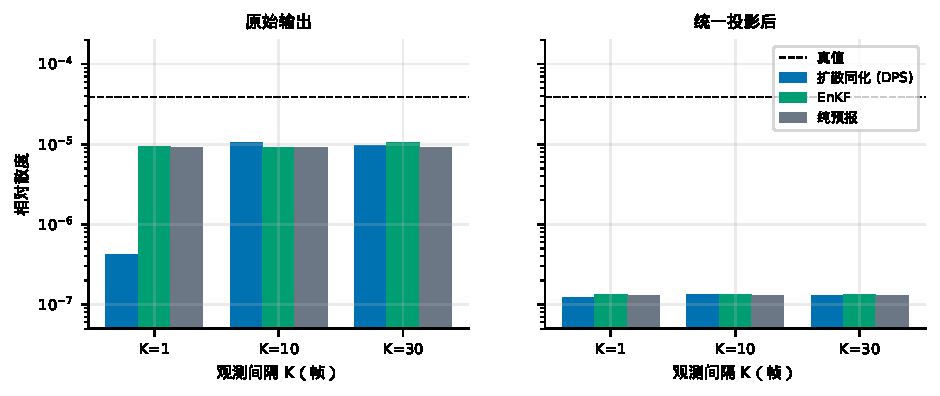
\includegraphics[width=\linewidth]{report_fig_main/div.pdf}\caption{同化结果的相对散度（虚线为真值的散度；第 40--99 帧，3 个种子、20 个轨迹平均）。}\end{figure}
$K=1$ 时扩散同化原始输出的散度（$4.2\times10^{-7}$）比 EnKF（$9.4\times10^{-6}$）低，这是因为扩散同化在输出前已做投影，EnKF 没有；对两者施加同一个投影后，散度相同（$1.2\times10^{-7}$ 对 $1.3\times10^{-7}$）。$K=20$ 时多数帧是求解器的预报输出，三种方法的散度都处在求解器输出自身的水平（约 $9.2\times10^{-6}$）。扩散模型的原始采样输出散度明显偏大，但投影对精度几乎没有影响：在 5 个验证轨迹（$K=1$，100 帧）上，不做投影时未观测点 RMSE 为 0.0158、原始散度 0.042，做投影后 RMSE 为 0.0157，5 个轨迹上投影后都略低（差 0.00004--0.00011）。

\subsection{小结}
(1) $K=1,5$ 时扩散同化的未观测点 RMSE 低于 EnKF，分别低 32\% 与 12\%。(2) $K=10,20$ 时 EnKF 更低，扩散同化的 RMSE 分别高 13\% 与 22\%；EnKF 的初始集合取自测试轨迹真值的前 20 帧。(3) 各 $K$ 下两种同化方法都低于纯预报。(4) 投影后，扩散同化与 EnKF 的散度相同。
\end{document}
